\section{系统设计}

AquaFS 是一个模块化的文件系统,以下是 AquaFS 的整体架构图:

\subsection{AquaFS 整体架构}

\begin{figure}[H]
    \centering
    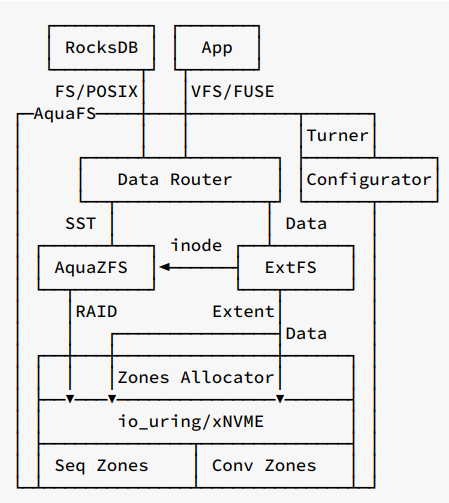
\includegraphics[width=0.8\textwidth]{fig/aquafs-frame.png}
    \caption{AquaFS 整体架构图}
    \label{aquafs-frame}
\end{figure}

架构图 \ref{aquafs-frame} 中的模块简略说明如下:

\begin{enumerate}
    \item App:文件系统请求负载
    \item RocksDB:数据库请求
    \item Data Router:FileSystem 请求路由器,需要判断当前请求是否适合 WAL 优化
    \item Turner:动态调整运行过程中的参数
    \item Configurator:静态调整文件系统参数,建立文件系统时给出建议参数
    \item AquaZFS:经过修改和优化的 ZenFS,支持 RAID 等功能
    \item ExtFS:有 inode 系统的运行于 Seq/Conv Zones 上的通用文件系统
        \begin{enumerate}
            \item 对普通请求,直接使用 Conv Zones
            \item 对 AquaZFS 的新文件,提供 inode 索引等读写优化
            \item 对较大的冷数据文件,分配到 Seq Zones
            \item 将一些可以异地更新的数据以 AquaFS::Extent 形式写入 AquaZFS
        \end{enumerate}
    \item Zones Allocator:为 AquaZFS、ExtFS 提供 Zone 分配服务
    \item Zones:
        \begin{enumerate}
            \item Seq Zones:只能顺序写的 Zones
            \item Conv Zones:可以随机写的 Zones
        \end{enumerate}
    \item AquaFS:整体文件系统
\end{enumerate}

\subsection{模块设计细节}

\subsubsection*{RocksDB 使用 AquaFS}

RocksDB 使用 AquaFS,可以走两种数据通路:FileSystem 和 POSIX 接口。

\textbf{RocksDB 使用 FileSystem 接口使用 AquaFS}

将 AquaFS 编译为 RocksDB 插件,Data Router 使用 FileSystem 接口。

Data Router 主要转发 SST 请求到 AquaZFS,其他请求转发到 ExtFS,并对特殊情况做二者的负载均衡。

\textbf{RocksDB 使用 POSIX 接口使用 AquaFS}

AquaFS 的 Data Router 通过 Kernel Module 或 FUSE 提供 POSIX 访问接口,并智能判断数据负载位置。

\subsubsection*{App 使用 AquaFS}

由于假定 App 并未实现 FileSystem 接口,所以 App 数据可以通过 Kernel Module / FUSE 方式经过 Data Router 到下层。

\subsubsection*{调参模块}

AquaFS 中调参模块主要有两个部分:Configurator、Turner。

Configurator 在文件系统创建前评估当前系统更适合的固定参数,并结合需求给出合适的参数选择和预估的性能区间。

Turner 在文件系统使用过程中保持运行,根据系统当前状态动态调整可改变的参数,以获得更加灵活良好的整体表现。

\textbf{可调参数}

\begin{enumerate}
    \item 固定参数
    \begin{enumerate}
        \item 块大小
        \item 固定 RAID 参数
        \item 数据后端类型
    \end{enumerate}
    \item GC
    \begin{enumerate}
        \item GC 容量阈值
        \item GC 间隔时间
    \end{enumerate}
    \item 动态 RAID
    \begin{enumerate}
        \item 分配时间(GC)
        \item 分配参数(0/1/5...)
    \end{enumerate}
    \item 文件请求分类
    \begin{enumerate}
        \item 分类为 SST、普通数据
        \item 分类冷热文件/数据
    \end{enumerate}
    \item IO 加速方式:io\_uring/xNVME
\end{enumerate}

\subsubsection*{AquaZFS 和 ExtFS}

ExtFS 是主要运行于 Conv Zones 上的针对 ZNS 优化的文件系统。主要特性:

\begin{enumerate}
    \item 必须原地更新的数据放在 Conv Zones 内,如 Superblock 等(?)
    \item 适合异地更新的数据通过 AquaZFS 保存在 Seq Zones 内,如 MetaData(?)
    \item 如果智能检测到 AquaZFS 内部分数据不适合 Seq Zones 存储,则转发到 ExtFS 内处理
    \item 用冗余的 inode 等为 AquaZFS 提供索引,可以动态降低其内存消耗
\end{enumerate}

AquaZFS 是基于 ZenFS 的优化修改,支持以上特性,在保存高性能的同时提升文件系统的灵活性。

\subsubsection*{RAID}

在 AquaZFS 从写盘前到实际写盘之间,存在一层 RAID 逻辑。

在原版 ZenFS 的实现中并没有实现 RAID 的逻辑,其只能保证存储的“记录”的数据正确性,而无法保证“文件”的数据正确性,
也不能在遇到磁盘故障的时候自动处理修复数据。

AquaZFS 在 ZenFS 的基础上实现了 RAID 逻辑,可以在磁盘故障时自动修复数据,且能够根据配置自动使用不同的 RAID 策略。

除了保证数据的正确性,AquaZFS 还可以根据不同的 RAID 策略提供不同的性能。
当前实现的 RAID0 可以以 N 倍加速单线程数据的读写,RAID1 在提供 N 倍读性能的同时,还可以用简单的冗余策略保证数据的安全性。

AquaZFS 的 RAID 有两种基本模式:全盘模式和智能动态分区模式。

在全盘模式下,AquaZFS 会以 SSD 设备为单位应用同一种 RAID 策略,其策略配置写入超级块中,
可以快速将已经在使用的 AquaZFS 转换为 全盘 RAID 格式,并使用超级块在 Meta Zones 中的追加写入逻辑保证配置的正确性。

在智能动态分区模式下,AquaZFS 以 Zones 为单位配置 RAID 策略,可以在不同的 Zones 中使用不同的 RAID 策略。
RAID 策略信息以记录形式写入 Meta Zones 中,并使用 WAL 配合 Snapshot 保证数据的正确性。

在实现的过程中,我们为其他的 RAID 逻辑做了预留,能够快速地实现其他 RAID 逻辑。

\begin{enumerate}
    \item 可灵活配置为:静态固定参数 RAID、智能动态分区 RAID
    \item 可以在用户态驱动 NVME,或者内核态使用 liburing 进行 IO 加速,充分利用多盘优势提升性能
    \item 利用 Turner 提供的建议,在 AquaZFS 垃圾回收时或合并 Extent 时调整 RAID 逻辑,使文件系统在安全性、性能上有更好的权衡点
\end{enumerate}

\subsubsection*{Zones Allocator}

为 AquaZFS 和 ExtFS 提供统一的 Zones 分配服务。

\begin{enumerate}
    \item 让整盘空间得到更加充分的利用,减少由于分开两种子系统造成的空间碎片
    \item 根据历史数据,测算不同 Zones 的寿命和速度,来控制 Zones 的分配逻辑,延长磁盘寿命,提高磁盘吞吐
\end{enumerate}

\subsubsection*{IO 加速}

在 AquaFS 向上提供 FileSystem 接口时,由于负载程序对 FileSystem 接口做了适配,所以可以让负载程序和整个 AquaFS 都跑在用户态。

当 AquaFS 整个运行在用户态,可以使用 xNVME 用户态 NVME 协议驱动,降低内核态用户态切换的性能损失,同时也可用 io\_uring 加速。

若 AquaFS 使用 POSIX 接口,可以使用 VFS 或者 FUSE 接口,此时也可以用 xNVME 或者 io\_uring 进行 IO 加速。

\subsubsection*{智能化}

这个架构的「智能」体现在哪?

\begin{enumerate}
    \item 相比与 ZenFS,灵活性更强
    \begin{enumerate}
        \item 适配没有针对优化的工作负载,智能识别适合 WAL 的数据,用更合适的方式处理
        \item 可调整的静态、动态参数更多
        \item 提供 RAID 功能,并可以动态分配
    \end{enumerate}
    \item 数据安全性更强:RAID 功能
    \item 智能分配请求
    \begin{enumerate}
        \item 在 Data Router 层合理分配 SST、普通数据请求
        \item 在当前请求不适合 AquaZFS 的时候将 ExtFS 作为后备
        \item 进行读写请求分离
    \end{enumerate}
\end{enumerate}

